\chapter[TorchIO: a software library for medical image processing]{TorchIO: a software library for medical image preprocessing and augmentation in deep learning}
% {TorchIO: a Python library for efficient loading, preprocessing, augmentation and patch-based sampling of medical images in deep learning}

\chaptermark{TorchIO: a library for medical image processing}
\label{chap:torchio}
\minitoc

\begin{center}
  \begin{minipage}[b]{0.9\linewidth}
    \small
    \textbf{Foreword\,}
    This chapter is an \textit{in extenso} reproduction of:
    \begin{itemize}
      \item \bibentry{perez-garcia_torchio_2021}
    \end{itemize}
  \end{minipage}
\end{center}

\section{Introduction}

\subsection{Motivation}

Approximately one third of epilepsies are drug-resistant.
If the \ac{EZ}, i.e., ``the area of cortex indispensable for the generation of clinical seizures'' \cite{rosenow_presurgical_2001}, can be localized, resective surgery to remove the \ac{EZ} may be curative.
As previously mentioned, only 40\% to 70\% of patients with refractory focal epilepsy are seizure-free after surgery \cite{jobst_resective_2015}.
This is, in part, due to limitations identifying the \ac{EZ} during the presurgical evaluation.
Retrospective studies relating presurgical clinical features and resected brain structures to surgical outcome provide useful insights to guide \ac{EZ} resection \cite{jobst_resective_2015}.
To quantify resected structures, first, the \ac{RC} must be segmented on the postoperative \ac{MRI}.
A preoperative image with a corresponding brain parcellation can then be registered to the postoperative \ac{MRI} to identify resected structures.

\Ac{RC} segmentation is also necessary in other applications.
For neuro-oncology, the gross tumor volume, which is the sum of the \ac{RC} and residual tumor volumes, is estimated for postoperative radiotherapy \cite{ermis_fully_2020}.

Despite recent efforts to segment \acp{RC} in the context of brain cancer \cite{meier_automatic_2017,ermis_fully_2020}, little research has been published in the context of epilepsy surgery.
Furthermore, previous work is limited by the lack of benchmark datasets, released code or trained models, and evaluation is restricted to single-institution datasets used for both training and testing.


\subsection{Related works}

After surgery, \acp{RC} fill with \ac{CSF}.
This causes an inherent uncertainty in delineating \acp{RC} adjacent to structures such as sulci, ventricles or edemas.
Nonlinear registration has been presented to segment the \ac{RC} for epilepsy \cite{chitphakdithai_non-rigid_2010} and brain tumor \cite{chen_deformable_2015} surgeries by detecting non-corresponding regions between pre- and postoperative images.
However, evaluation of these methods was restricted to a very small number of images.
Furthermore, in cases with intensity changes due to the resection (e.g., brain shift, atrophy, fluid filling), non-corresponding voxels may not correspond to the \ac{RC}.

Decision forests were presented for brain cavity segmentation after glioblastoma surgery, using four \ac{MRI} modalities \cite{meier_automatic_2017}.
These methods, which aggregate hand-crafted features extracted from all  modalities to train a classifier, can be sensitive to signal inhomogeneity and unable to distinguish regions with intensity patterns similar to \ac{CSF} from \acp{RC}.
Recently, a 2D \ac{CNN} was trained to segment the \ac{RC} on \ac{MRI} slices in 30 glioblastoma patients \cite{ermis_fully_2020}.
They obtained a `median (interquartile range)' \ac{DSC} of 84 (10) compared to ground-truth labels by averaging predictions across anatomical axes to compute the 3D segmentation.
While these approaches require four modalities to segment the \ac{RC}, some of the modalities are often unavailable in clinical settings \cite{dorent_learning_2021}.
Furthermore, code and datasets are not publicly available, hindering a fair comparison across methods.
Applying these techniques requires curating a dataset with manually obtained annotations to train the models, which is expensive.

Unsupervised learning methods can leverage large, unlabeled medical image datasets during training.
In self-supervised learning, training instances are generated automatically from unlabeled data and used to train a model to perform a pretext task. %such as inpainting or image restoration.
The model can be fine-tuned on a smaller labeled dataset to perform a downstream task \cite{chen_self-supervised_2019}.
The pretext and downstream tasks may be the same.
For example, a \ac{CNN} was trained to reconstruct a skull bone flap by simulating craniectomies on CT scans \cite{matzkin_self-supervised_2020}.
Lesions simulated in chest CT of healthy subjects were used to train models for nodule detection, improving accuracy compared to training on a smaller dataset of real lesions \cite{pezeshk_seamless_2017}.

% Recovered from long version
Semi-supervised learning may be used when a large amount of unlabeled data is available.
A model trained on a labeled dataset (which may have been generated in a self-supervised setting) can generate pseudolabels for unlabeled data.
Uncertainty estimation may be used to select pseudolabeled instances with a low uncertainty for medical image segmentation tasks, improving model performance compared to using a random subset \cite{venturini_uncertainty_2020}.


\subsection{Contributions}

We present a self-supervised learning approach to train a 3D \ac{CNN} for brain \acp{RC} segmentation from \ac{T1w} \ac{MRI} without annotated data, by simulating resections during training.
We performed a comprehensive evaluation of our framework, assessing the effect of the resection simulation shape on performance and evaluating datasets from different institutions and pathologies.
We used uncertainty estimation as a selection criterion for pseudolabeled instances within our semi-supervised learning setting, which can be leveraged when postoperative \acp{MRI} without annotation are available, a typical scenario in clinical settings.

We ensure our work is reproducible by releasing the source code for resection simulation and \ac{CNN} training, the trained \ac{CNN}, and the evaluation dataset.
To the best of our knowledge, we introduce the first open annotated dataset of postoperative \ac{MRI} for epilepsy surgery.

\subsection{Motivation}

The nature of medical images makes it difficult to rely on a typical computer-vision pipeline for neural network training.
In \cref{sec:challenges}, we describe challenges related to medical images that need to be overcome when designing deep learning workflows.
In \cref{sec:frameworks}, we justify the choice of PyTorch as the main deep learning framework dependency of TorchIO.

\subsubsection{Challenges in medical image processing for deep learning}
\label{sec:challenges}


In practice, multiple challenges must be addressed when developing deep learning algorithms for medical images:
1) handling metadata related to physical position and size,
2) lack of large labeled datasets,
3) high computational costs due to data multidimensionality and
4) lack of consensus for best normalization practices.
These challenges are very common in medical imaging and require certain features that may not be implemented in more general-purpose image processing frameworks such as Albumentations~\cite{buslaev_albumentations_2020} or TorchVision~\cite{paszke_pytorch_2019}.


\paragraph{Metadata}
\label{sec:metadata}

In computer vision, picture elements, or \textit{pixels}, which are assumed to be square, have a spatial relationship that comprises proximity and depth according to both the arrangement of objects in the scene and camera placement.
In comparison, medical images are reconstructed such that the location of volume elements, or cuboid-shaped \textit{voxels}, encodes a meaningful 3D spatial relationship.
In simple terms, for 2D natural images, pixel vicinity does not necessarily indicate spatial correspondence, while for medical images spatial correspondence between nearby voxels can often be assumed.

Metadata, which encodes the physical size, spacing, and orientation of voxels, determines spatial relationships between voxels~\cite{larobina_medical_2014}.
This information can provide meaningful context when performing medical image processing, and is often implicitly or explicitly used in medical imaging software.
Furthermore, metadata is often used to determine correspondence between images as well as voxels within an image.
For example, registration algorithms for medical images typically work with physical coordinates rather than voxel indices.

\cref{fig:metadata} shows the superposition of an \ac{MRI} and a corresponding brain parcellation~\cite{cardoso_geodesic_2015} with the same size ($181 \times 181$) but different origin, spacing and orientation.
A naïve user would assume that, given that the superimposition looks correct and both images have the same size, they are ready for training.
However, the visualization is correct only because 3D Slicer~\cite{fedorov_3d_2012}, the software used for visualization, is aware of the spatial metadata of the images.
As \acp{CNN} generally do not take spatial metadata into account, training using these images without preprocessing would lead to poor results.


\begin{figure}
  \centering

  \begin{subfigure}{0.24\textwidth}
    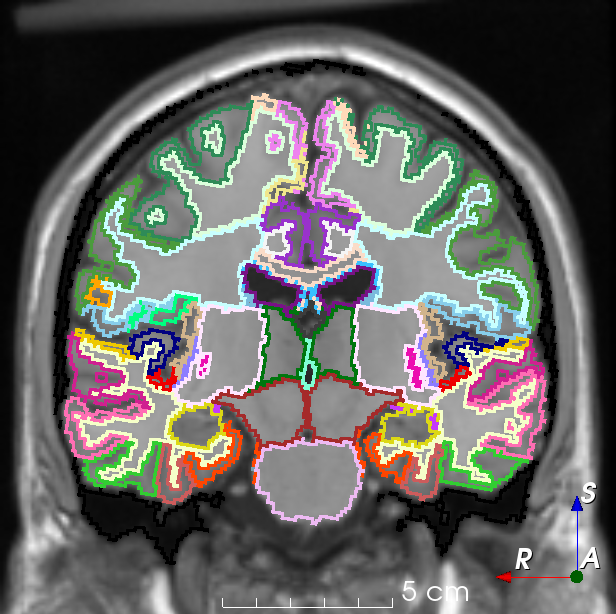
\includegraphics[width=\linewidth]{metadata_ok}
    \caption{}
    \label{fig:meta_ok}
  \end{subfigure}
  \hfill
  \begin{subfigure}{0.24\textwidth}
    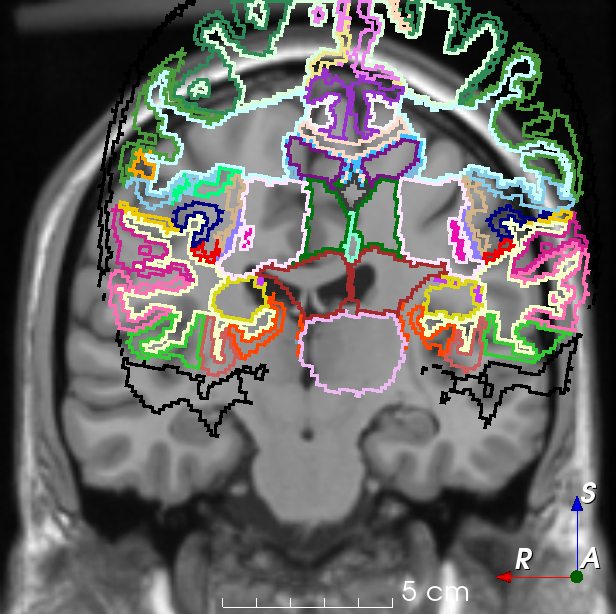
\includegraphics[width=\linewidth]{metadata_origin}
    \caption{}
    \label{fig:meta_origin}
  \end{subfigure}
  \hfill
  \begin{subfigure}{0.24\textwidth}
    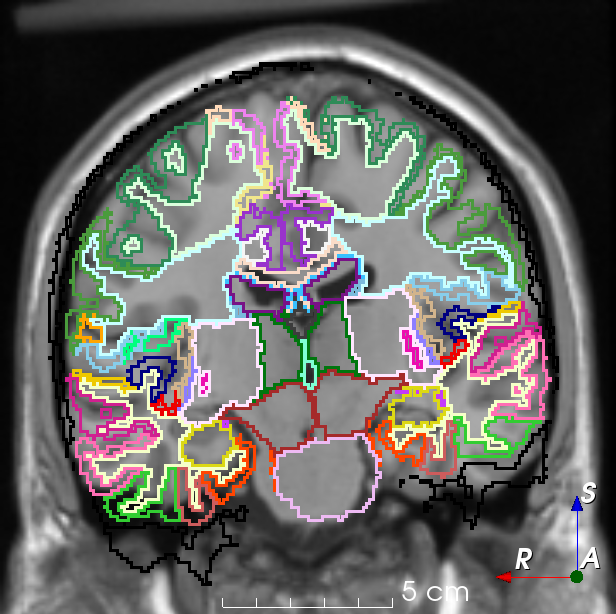
\includegraphics[width=\linewidth]{metadata_orientation}
    \caption{}
    \label{fig:meta_orientation}
  \end{subfigure}
  \hfill
  \begin{subfigure}{0.24\textwidth}
    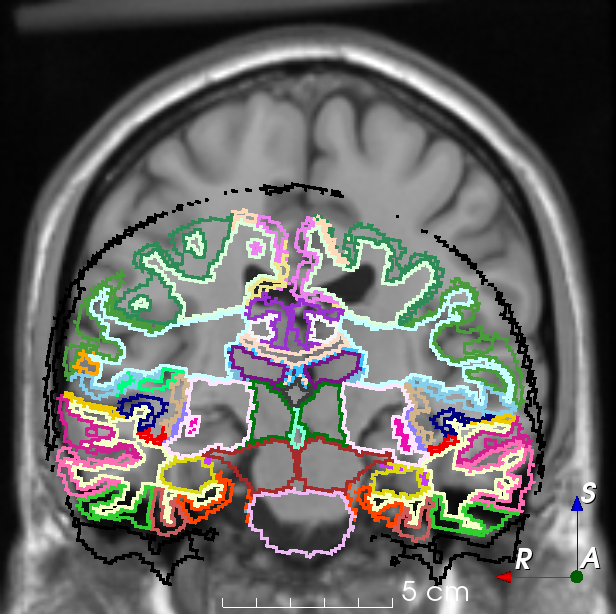
\includegraphics[width=\linewidth]{metadata_spacing}
    \caption{}
    \label{fig:meta_spacing}
  \end{subfigure}

  \caption[Importance of spatial metadata in medical imaging processing]{
    Demonstration of the importance of spatial metadata in medical image processing.
    The size of both the \ac{MRI} and the segmentation is $181 \times 181$.
    When spatial metadata is taken into account (\subref{fig:meta_ok}), images are correctly superimposed (only the borders of each region are shown for clarity purposes).
    Images are incorrectly superimposed if (\subref{fig:meta_origin}) origin, (\subref{fig:meta_orientation}) orientation or (\subref{fig:meta_spacing}) spacing are ignored.
  }
  \label{fig:metadata}
\end{figure}



Medical images are typically stored in specialized formats such as \ac{DICOM} or \ac{NIfTI}~\cite{larobina_medical_2014}, and commonly read and processed by medical imaging frameworks
such as SimpleITK~\cite{lowekamp_design_2013} or NiBabel~\cite{brett_nipynibabel_2020}.


\paragraph{Limited training data}

Deep learning methods typically require large amounts of annotated data, which are often scarce in clinical scenarios due to concerns over patient privacy, the financial and time burden associated with collecting data as part of a clinical trial, and the need for annotations from highly-trained and experienced raters.
Data augmentation techniques can be used to increase the size of the training dataset artificially by applying different transformations to each training instance while preserving the relationship to annotations.

Data augmentation performed in computer vision typically aims to simulate variations in camera properties, \ac{FOV}, or perspective.
Traditional data augmentation operations applied in computer vision include geometrical transforms such as random rotation or zoom, color-space transforms such as random channel swapping or kernel filtering such as random Gaussian blurring.
Data augmentation is usually performed on the fly, i.e., every time an image is loaded from disk during training.

Several computer vision libraries supporting data augmentation have appeared recently, such as Albumentations~\cite{buslaev_albumentations_2020}, or \texttt{imgaug}~\cite{jung_imgaug_2020}.
PyTorch also includes some computer vision transforms, mostly implemented as Pillow wrappers~\cite{wiredfool_pillow_2016}.
However, none of these libraries support reading or transformations for 3D images.
Furthermore, medical images are almost always greyscale, therefore colour-space transforms are not applicable.
Additionally, cropping and scaling are more challenging to apply to medical images without affecting the spatial relationships of the data.
Metadata should usually be considered when applying these transformations to medical images.

In medical imaging, the purpose of data augmentation is designed to simulate anatomical variations and scanner artifacts.
Anatomical variation and sample position can be simulated using spatial transforms such as elastic deformation, lateral flipping, or affine transformations.
Some artifacts are unique to specific medical image modalities.
For example, ghosting artifacts will be present in \ac{MRI} if the patient moves during acquisition, and metallic implants often produce streak artifacts in \ac{CT}.
Simulation of these artifacts can be useful when performing augmentation on medical images.


\paragraph{Computational costs}
\label{sec:computation}
The number of pixels in 2D images used in deep learning is rarely larger than one million.
For example, the input size of several popular image classification models is $224 \times 224 \times 3 = \num{150528}$ pixels (\SI{588}{\kibi\byte} if 32 bits per pixel are used).
In contrast, 3D medical images often contain hundreds of millions of voxels, and downsampling might not be acceptable when small details should be preserved.
For example, the size of a high-resolution lung \ac{CT}-scan used for quantifying chronic obstructive pulmonary disease damage in a research setting, with spacing $0.66 \times 0.66 \times 0.30$ mm, is $512 \times 512 \times 1069 = \num{280231936}$ voxels (\SI{1.04}{\gibi\byte} if 32 bits per voxel are used).


In computer vision applications, images used for training are grouped in batches whose size is often in the order of hundreds~\cite{krizhevsky_imagenet_2012} or even thousands~\cite{chen_simple_2020} of training instances, depending on the available \ac{GPU} memory.
In medical image applications, batches rarely contain more than one~\cite{cicek_3d_2016} or two~\cite{milletari_v-net_2016} training instances due to their larger memory footprint compared to natural images.
This reduces the utility of techniques such as batch normalization, which rely on batches being large enough to estimate dataset variance appropriately~\cite{ioffe_batch_2015}.
Moreover, large image size and small batches result in longer training time, hindering the experimental cycle that is necessary for hyperparameter optimisation.
In cases where \ac{GPU} memory is limited and the network architecture is large, it is possible that not even the entirety of a single volume can be processed during a training iteration.
To overcome this challenge, it is common in medical imaging to train using subsets of the image, or image \textit{patches}, randomly extracted from the volumes.

Networks can be trained with 2D slices extracted from 3D volumes, aggregating the inference results to generate a 3D volume~\cite{lucena_convolutional_2019}.
This can be seen as a specific case of patch-based training, where the size of the patches along a dimension is one.
Other methods extract volumetric patches for training, that are often cubes, if the voxel spacing is isotropic~\cite{li_compactness_2017}, or cuboids adapted to the anisotropic spacing of the training images~\cite{nikolov_deep_2018}.


\paragraph{Transfer learning and normalization}

One can pre-train a network on a large dataset of natural images such as ImageNet~\cite{deng_imagenet_2009}, which contains more than 14 million labeled images, and fine-tune on a custom, much smaller target dataset.
This is a typical use of transfer learning in computer vision~\cite{weiss_survey_2016}.
The literature has reported mixed results using transfer learning to apply models pretrained on natural images to medical images~\cite{cheplygina_cats_2019,raghu_transfusion_2019}.

In computer vision, best practice is to normalize each training instance before training, using statistics computed from the whole training dataset~\cite{krizhevsky_imagenet_2012}.
Preprocessing of medical images is often performed on a per-image basis, and best practice is to take into account the bimodal nature of medical images (i.e., that an image has a background and a foreground).

Medical image voxel intensity values can be encoded with different data types and intensity ranges, and the meaning of a specific value can vary between different modalities, sequence acquisitions, or scanners.
Therefore, intensity normalization methods for medical images often involve more complex parameterization of intensities than those used for natural images~\cite{nyul_standardizing_1999}.

\subsubsection{Deep learning frameworks}
\label{sec:frameworks}

There are currently two major generic deep learning frameworks: TensorFlow \cite{abadi_tensorflow_2016} and PyTorch \cite{paszke_pytorch_2019}, primarily maintained by Google and Facebook, respectively.
Although TensorFlow has traditionally been the primary choice for both research and industry, PyTorch has recently seen a substantial increase in popularity, especially among the research community \cite{he_state_2019}.

PyTorch is often preferred by the research community as it is \textit{pythonic}, i.e., its design, usage, and \ac{API} follow the conventions of plain Python. Moreover, the \ac{API} for tensor operations follows a similar paradigm to the one for NumPy multidimensional arrays, which is the primary array programming library for the Python language \cite{van_der_walt_numpy_2011}.
In contrast, for TensorFlow, researchers need to become familiar with new design elements such as sessions, placeholders, feed dictionaries, gradient tapes and static graphs.
In PyTorch, objects are standard Python classes and variables, and a dynamic graph makes debugging intuitive and familiar to anyone already using Python.
These differences have decreased with the recent release of TensorFlow 2, whose eager mode makes usage reminiscent of Python.

TorchIO was designed to be in the style of PyTorch and uses several of its tools to reduce the barrier to learning how to use TorchIO for those researchers already familiar with PyTorch.


\subsection{Related work}

NiftyNet \cite{gibson_niftynet_2018} and the \ac{DLTK} \cite{pawlowski_dltk_2017} are deep learning frameworks designed explicitly for medical image processing using the TensorFlow~1 platform.
Both of them are no longer being actively maintained.
They provide implementations of some popular network architectures such as U-Net \cite{cicek_3d_2016}, and can be used to train 3D \acp{CNN} for different tasks.
For example, NiftyNet was used to train a 3D residual network for brain parcellation \cite{li_compactness_2017}, and \ac{DLTK} was used to perform multi-organ segmentation on \ac{CT} and \ac{MRI} \cite{valindria_multi-modal_2018}.

The \texttt{medicaltorch} library \cite{christian_s_perone_peronemedicaltorch_2018} closely follows the PyTorch design, and provides some functionalities for preprocessing, augmentation and training of medical images.
However, it does not leverage the power of specialized medical image processing libraries, such as SimpleITK \cite{lowekamp_design_2013}, to process volumetric images.
Similar to \ac{DLTK}, this library has not seen much activity since 2018.

The \texttt{batchgenerators} library \cite{isensee_batchgenerators_2020}, used within the popular medical segmentation framework nn-UNet \cite{isensee_nnu-net_2021}, includes custom dataset and data loader classes for multithreaded loading of 3D medical images, implemented before data loaders were available in PyTorch.
In the usage examples from GitHub, preprocessing is applied to the whole dataset before training.
Then, spatial data augmentation is performed at the volume level, from which one patch is extracted and intensity augmentation is performed at the patch level.
In this approach, only one patch is extracted per volume, diminishing the efficiency of training pipelines.
Transforms in \texttt{batchgenerators} are mostly implemented using NumPy \cite{van_der_walt_numpy_2011} and SciPy \cite{virtanen_scipy_2020}.

More recently, a few PyTorch-based libraries for deep learning and medical images have appeared.
There are two other libraries, developed in parallel to TorchIO, focused on data preprocessing and augmentation.
Rising\fnurl{https://github.com/PhoenixDL/rising} is a library for data augmentation entirely written in PyTorch, which allows for gradients to be propagated through the transformations and perform all computations on the \ac{GPU}.
However, this means specialized medical imaging libraries such as SimpleITK cannot be used.
\texttt{pymia} \cite{jungo_pymia_2021} provides features for data handling (loading, preprocessing, sampling) and evaluation.
It is compatible with TorchIO transforms, which are typically leveraged for data augmentation, as their data handling is more focused on preprocessing.
\texttt{pymia} can be easily integrated into either PyTorch or TensorFlow pipelines.
It was recently used to assess the suitability of evaluation metrics for medical image segmentation \cite{kofler_are_2021}.

\ac{MONAI} \cite{nic_ma_project-monaimonai_2021} and Eisen \cite{mancolo_eisen_2020} are PyTorch-based frameworks for deep learning workflows with medical images.
Similar to NiftyNet and \ac{DLTK}, they include implementation of network architectures, transforms, and higher-level features to perform training and inference.
For example, \ac{MONAI} was recently used for brain segmentation on fetal \ac{MRI} \cite{ranzini_monaifbs_2021}.
As these packages are solving a large problem, i.e., that of workflow in deep learning for medical images, they do not contain all of the data augmentation transforms present in TorchIO.
However, it is important to note that an end user does not need to select only one open-source package, as TorchIO transforms are compatible with both Eisen and \ac{MONAI}.

TorchIO is a library that specializes in preprocessing and augmentation using PyTorch, focusing on ease of use for researchers.
This is achieved by providing a PyTorch-like \ac{API}, comprehensive documentation with many usage examples, and tutorials showcasing different features, and by actively addressing feature requests and bug reports from the many users that have already adopted TorchIO.
This is in contrast with other modern libraries released after TorchIO such as \ac{MONAI}, which aims to deliver a larger umbrella of functionalities including federated learning or active learning, but may have slower development and deployment.

\section{Methods}
\label{sec:methods}

\newcommand{\p}{\bm{p}}
\newcommand{\vv}{\bm{v}}
\newcommand{\X}{\bm{X}}
\newcommand{\Y}{\bm{Y}}
\newcommand{\M}{\bm{M}}
\newcommand{\U}{\bm{U}}
% \newcommand{\R}{\mathbb{R}}

\newcommand{\img}[2]{#1 : \Omega \to #2}
\newcommand{\binimg}[1]{\img{#1}{ \{ 0, 1 \} }}

\newcommand{\Dom}{\mathcal{D}}
\newcommand{\Tas}{\mathcal{T}}
\newcommand{\Xdo}{\mathcal{X}}
\newcommand{\Ydo}{\mathcal{Y}}
\newcommand{\fp}[1]{f_{\theta \text{#1}}}
\newcommand{\wt}{\widetilde}

% https://tex.stackexchange.com/a/466437/216202
\renewcommand*\st[1]{_{\textnormal{#1}}}

\newcommand{\post}{\st{postop}}
\newcommand{\pre}{\st{preop}}
\newcommand{\cav}{\st{cavity}}
\newcommand{\simul}{\st{sim}}
\newcommand{\lab}{\st{labeled}}
\newcommand{\unl}{\st{unlabeled}}


We describe our learning strategy in \cref{sec:learning_strategy} (\cref{fig:diagram_ijcars})
and introduce our \ac{RC} simulation in \cref{sec:simulation}.

\begin{figure}[ht]
  \centering
  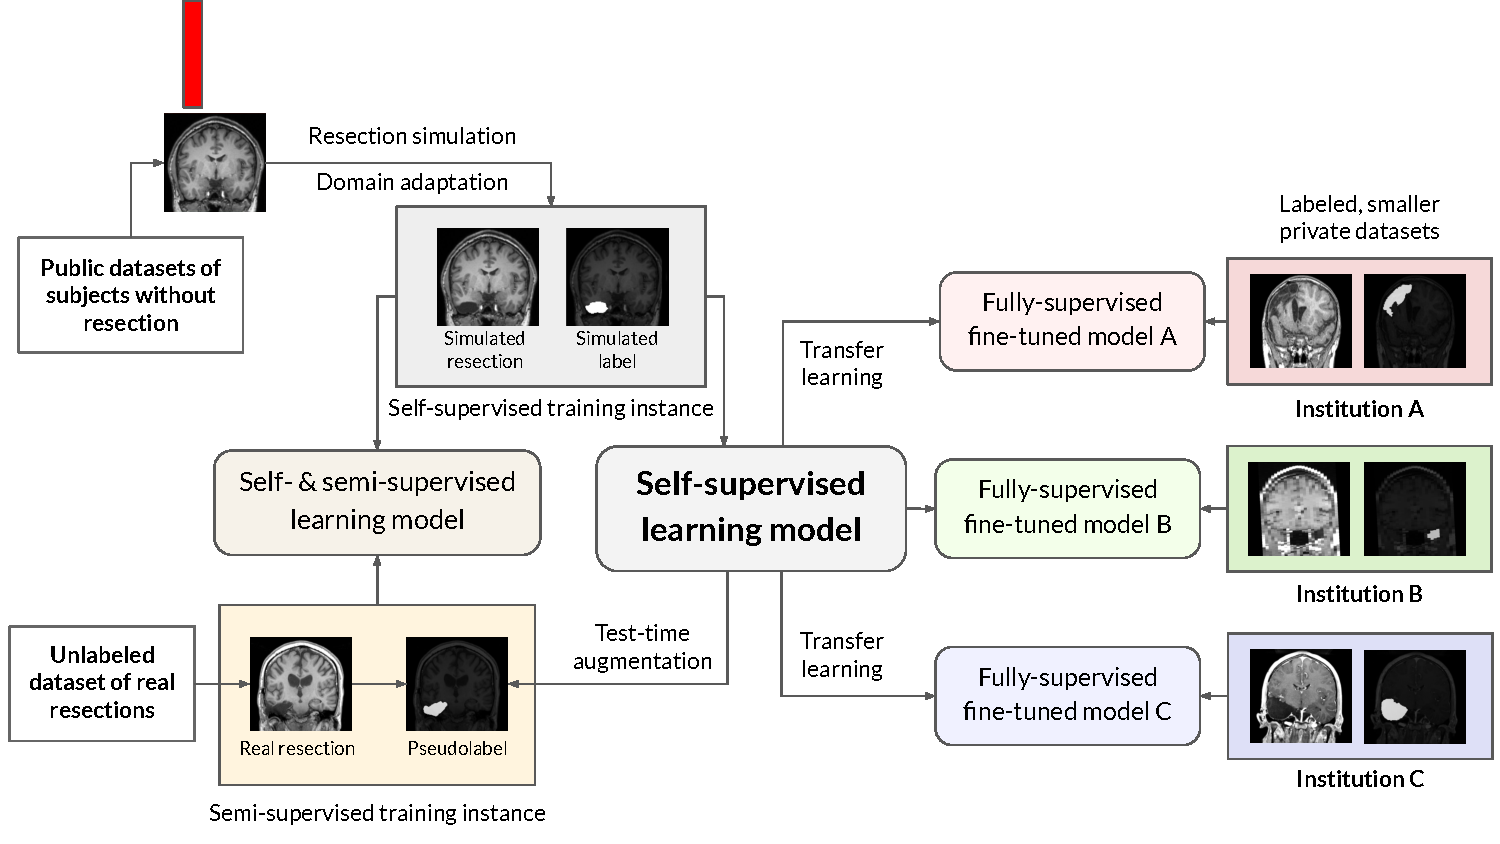
\includegraphics[trim={0 0 0 52},clip, width=\linewidth]{diagram_ijcars}
  \caption[Learning strategies for cavity segmentation]{
    Learning strategies.
    3D images without resections (top left) are modified by our resection simulation method to mimic postoperative images and their corresponding labels, generating training instances.
    These instances are used to train a baseline model in a self-supervised manner (middle).
    The baseline model generates pseudolabels from unlabeled images of patients who underwent resective surgery (bottom left).
    Instances from the \ac{RC} simulation and pseudolabeled dataset are used to train a new model in a self- and semi-supervised learning approach (left).
    The baseline model may be fine-tuned to improve its performance on small labeled datasets containing real resections from a single institution, using a standard fully-supervised learning approach (right).
  }
  \label{fig:diagram_ijcars}
\end{figure}

\subsection{Learning strategy}
\label{sec:learning_strategy}


\subsubsection{Problem statement}

\newcommand{\loss}{\mathcal{L}}
\newcommand{\expec}{\mathbb{E}}
\newcommand{\exppost}{\expec_{\Dom\post}}

The overall objective is to automatically segment resection cavities from postoperative \ac{T1w} \ac{MRI} using a \ac{CNN} $f_{\bm{\theta}}$ parameterized by weights $\bm{\theta}$.
Let $\X_{\text{post}} : \Omega \to \R$ and $\Y\cav  : \Omega \to \{ 0, 1 \}$ be a postoperative \ac{T1w} \ac{MRI} and its cavity segmentation label, respectively, where $\Omega \subset \R^3$.
$\X_{\text{post}}$ and $\Y_{\text{cavity}}$ are drawn from the data distribution $\Dom\post$.
In model training, the aim is to minimize the expected discrepancy between the label $\Y\cav$ and network prediction $f_{\bm{\theta}}(\X\post)$.
Let $\loss$ be a loss function that estimates this discrepancy (e.g., Dice loss).
The optimization problem for the network parameters $\bm{\theta}$ is:
\begin{equation}
  \bm{\theta}^* =
  \argmin_{\bm{\theta}}
  \exppost \left[
    \loss \left(
      f_{\bm{\theta}} \left( \X\post \right),
      \Y\cav
    \right)
  \right]
  \label{eq:problem_optimization}
\end{equation}


In a fully-supervised setting, a labeled dataset $D\post = \{ (\X_{\text{post}_i}, \Y_{\text{cavity}_i}) \}_{i = 1}^{n\post}$ is employed to estimate the expectation defined in \cref{eq:problem_optimization} as:
\begin{equation}
  \exppost \left[
    \loss \left(
      f_{\bm{\theta}} \left( \X\post \right), \Y\cav
    \right)
  \right]
  \approx \frac{1}{n\post} \sum_{i=1}^{n\post} \loss(f_{\bm{\theta}}(\X_{\text{post}_i}), \Y_{\text{post}_i})
  \label{eq:problem_optimization_fully}
\end{equation}

In practice, \acp{CNN} typically require an annotated dataset with a large $n\post$ to generalize well for unseen instances.
However, given the time and expertise required to annotate scans, $n\post$ is often small.
We present a method to artificially increase $n\post$ by simulating postoperative \acp{MRI} and associated labels from preoperative scans.


\subsubsection{Simulation for domain adaptation and self-supervised learning}
\label{sec:sim_res_self}

Let $D\pre = \{ \X_{\text{pre}_i} \}_{i = 1}^{n\pre}$ be a dataset of preoperative \ac{T1w} \ac{MRI}, drawn from the data distribution $\Dom\pre$.
We propose to generate a simulated postoperative dataset $D\simul = \{ (\X_{\text{sim}_i}, \Y_{\text{sim}_i}) \}_{i = 1}^{n\simul}$ using the preoperative dataset $D\pre$.
Specifically, we aim to build a generative model $\phi\simul : \X\pre \mapsto (\X\simul, \Y\simul)$ that transforms preoperative images into simulated, annotated postoperative images that imitate instances drawn from the postoperative data distribution $\Dom\post$.
$D\simul$ can then be used to estimate the expectation in \cref{eq:problem_optimization}:
\begin{equation}
  \exppost \left[\
    \loss\left(
      f_{\bm{\theta}} \left(\X\post \right), \Y\cav \right)
    \right]
    \approx \frac{1}{n\simul}\sum_{i=1}^{n\simul} \loss(f_{\bm{\theta}}(\X_{\text{sim}_i}),  \Y_{\text{sim}_i})
  \label{eq:problem_optimization_sim}
\end{equation}

Simulated images can be generated from any unlabeled preoperative dataset.
Therefore, the size of the simulated dataset can be much greater than the annotated dataset $D\post$, i.e., $n\simul\gg n\post$.
The network parameters $\bm{\theta}$ can be optimized by minimizing \cref{eq:problem_optimization_sim} using stochastic gradient descent, leading to a trained predictive function $f_{\bm{\theta_}{\text{sim}}}$.
Finally, $f_{\bm{\theta_}{\text{sim}}}$ can be fine-tuned on $D\post$ to improve performance on the postoperative domain $\Dom\post$.

\subsubsection{Leveraging unlabeled data from the target domain}
\label{sec:leveraging_semi}

Let $D\unl = \{ \X_{\text{postop}_i} \}_{i = 1}^{n\st{unl}}$ be a dataset comprising $n\st{unl}$ unlabeled postoperative images.
We propose to leverage $D\unl$ to build a better predictive model than using simulated resections only, employing a semi-supervised learning approach.
First, pseudolabels for each image $\X\post \in D\unl$ can be generated with $f_{\theta_{\text{sim}}}$ using data distillation, i.e., ensembling multiple predictions from transformed versions of $\X\post$.
Using the multiple predictions generated for pseudolabels, we estimate image-level segmentation uncertainty so that only instances with high reliability are used for training.
Finally, simulated resection instances and the selected pseudolabeled instances are used to train a new model $f_{\theta_{\text{sim+unl}}}$ in a hybrid self- and semi-supervised setting.


\paragraph{Generating pseudolabels using data distillation}

Data distillation is a method that ensembles predictions from multiple transformations applied to data, using a single model \cite{radosavovic_data_2017}.
We use Monte Carlo simulation to generate each pseudolabel with \ac{TTA}, which can improve the performance of segmentation models \cite{wang_aleatoric_2019}.
Let $n\st{u}$ represent the total number of simulation runs.
In the $i$-th simulation run,
the \ac{TTA} intensity and spatial transforms $T_\alpha$ and $T_\beta$ (\cref{sec:preprocessing_augmentation}) are applied to $\X\post$.
$\fp{sim}$ is used to predict $\wt{\Y}_{\theta\alpha\beta}'$, the probability of each voxel belonging to the cavity in the transformed space.
Finally, $T_\beta^{-1}$ is used to transform $\wt{\Y}_{\theta\alpha\beta}'$ back onto the space of $\X\post$:
\begin{equation}
    \wt{\Y}'_{\text{cavity}_i}
    = T_\beta^{-1}
    \circ \fp{sim}
    \circ T_\beta
    \circ T_\alpha
    \circ \X\post
    = T_\beta^{-1} \left( \wt{\Y}_{\theta\alpha\beta}' \right)
\end{equation}

We ensure that $T_\beta$ is invertible by using diffeomorphic spatial transformations.
To preserve image quality and ensure that probabilities stay within $[0, 1]$, we use tricubic and trilinear interpolation for $T_\beta$ and $T_\beta^{-1}$, respectively.

Predictions $P = \{ \wt{\Y}'_{\text{cavity}_i} \}_{i=1}^{n\st{u}}$ are averaged to obtain $\img{\wt{\Y}\cav}{[0, 1]}$, and the corresponding binary pseudolabel $\binimg{\widetilde{\Y}\cav}$ is obtained applying a threshold of 0.5 to $\wt{\Y}'\cav$.


\paragraph{Uncertainty estimation as selection criterion for pseudolabeled instances}

Images in $D\unl$ might have artifacts that limit the quality of the segmentation or include \acp{RC} not modeled by $\phi\simul$.
The corresponding noisy pseudolabels would hinder training of machine learning models.

As $n\st{unl}$ might be large, rather than performing manual quality control to select pseudolabels with high reliability for training, we use uncertainty estimation as an automated selection criterion \cite{venturini_uncertainty_2020}.

We use $n\st{unc}$ \ac{TTA} predictions to estimate aleatoric uncertainty, which captures noise inherent in the observation \cite{kendall_what_2017}.
Aleatoric uncertainty can indicate segmentation quality and is a successful selection criterion of pseudolabels in semi-supervised learning settings for medical image segmentation \cite{wang_aleatoric_2019,venturini_uncertainty_2020}.

Let $L = \{ l_i \}_{i = 1}^{n\st{unc}}$ denote the set of (soft) volumes of the segmented cavity for each prediction, where $l_i$ is the sum of all probabilities in the $i$-th prediction $\wt{\Y}'_{\text{cavity}_i} \in P$.
We use the \ac{CQV} of the volumes \cite{zwillinger_crc_1999,wang_aleatoric_2019} to estimate the image-level uncertainty $u : L \to \left[0, 1\right]$:
\begin{equation}
    u = \frac{q_3 - q_1}{q_3 + q_1}
\end{equation}
where $q_1$ and $q_3$ are the first and third quartiles of $L$, respectively.
The \ac{CQV} is agnostic to the volume of the segmented \ac{RC} and therefore avoids bias introduced by naturally-occurring uncertainty along the resection boundaries \cite{jungo_analyzing_2020}.
Finally, training instances with an associated prediction uncertainty $u(f_{\theta\alpha\beta}, \X\post, n\st{unc})$ below a threshold $t\st{unc}$ are combined with self-labeled instances (\cref{sec:sim_res_self}) to train a new model.

\subsection{Resection simulation for self-supervised learning}
\label{sec:simulation}

\newcommand{\AAA}{\bm{A}}
\newcommand{\NN}{\mathcal{N}}


$\phi\simul$ takes images from $\Dom\pre$ to generate training instances by simulating a realistic shape, location and intensity pattern for the \ac{RC}.
We present simulation of cavity shape and label in \cref{sec:cavity,sec:cavity_constrain}, respectively.
In \cref{sec:texture_cavity}, we present our method to generate the resected image.


\subsubsection{Initial cavity shape}
\label{sec:cavity}

To simulate a realistic \ac{RC}, we consider its topological and geometric properties: it is a single volume with a non-smooth boundary.
We generate a geodesic polyhedron with frequency $f$ by subdividing the edges of an icosahedron $f$ times and projecting each vertex onto a parametric sphere with a unit radius centered at the origin.
This polyhedron models a spherical surface $S = \{ V, F \}$ with vertices
$
  V = \left\{
    \vv_i \in \R^3
  \right\}
  _{i = 1}^{n_V}
$
and faces
$
  F = \left\{
    \bm{f}_k \in \mathbb{N}^3
  \right\}
  _{k = 1}^{n_F}
$, where $n_V$ and $n_F$ are the number of vertices and faces, respectively.
%
Each face $\bm{f}_k = \{ i_1^k, i_2^k, i_3^k \}$ is a sequence of three non-repeated vertex indices.

To create a non-smooth surface, $S$ is perturbed with simplex noise \cite{perlin_improving_2002}, a procedural noise generated by interpolating pseudorandom gradients on a multidimensional simplicial grid.
We chose simplex noise as it simulates natural-looking textures or terrains and is computationally efficient for multiple dimensions.
The noise $\eta : \R^3 \to [-1, 1]$ at point $\p \in \R^3$ is a weighted sum of the noise contribution for $\omega$ different octaves, with weights $\{\gamma ^ {n - 1}\}_{n = 1}^{\omega}$ controlled by the persistence parameter $\gamma$.
The displacement $\delta$ of a vertex $\vv$ is:
\begin{equation}
  \delta(\vv)
  = \eta \left( \frac{\vv + \bm{\mu} }{\zeta}, \omega, \gamma \right)
\end{equation}
where
$\zeta$ is a scaling parameter to control smoothness
and $\bm{\mu}$ is a shifting parameter that adds stochasticity
(equivalent to a random number generator seed).
%
Each vertex $\vv_i$ is displaced radially to create a perturbed sphere:
$
V_{\delta}
  = \left\{
  \vv_i
  + \delta(\vv_i)
  \frac{\vv_i}{\|\vv_i\|}
  \right\}
  _{i = 1}^{n_V}
  = \left\{
  \vv_{\delta i}
  \right\}
  _{i = 1}^{n_V}
$.

Next, a series of transforms is applied to $V_{\delta}$ to modify the mesh's volume and shape.
To add stochasticity, random rotations around each axis are applied to $V_{\delta}$ with the rotation transform
$T\st{R}(\bm{\theta}\st{r}) = R_x(\theta_x) \circ R_y(\theta_y) \circ R_z(\theta_z)$,
where~$\circ$~indicates a transform composition and
$R_i(\theta_i)$ is a rotation of $\theta_i$ radians around axis $i$.
$T\st{S}(\bm{r})$ is a scaling transform,
where $(r_1, r_2, r_3) = \bm{r}$ are semiaxes of an ellipsoid
with volume $v$ used to model the cavity shape.
The semiaxes are computed as
$r_1 = r$, $r_2 = \lambda r$ and $r_3 = r /\lambda$,
where $r = (3 v / 4)^{1/3}$ and
$\lambda$ controls the semiaxes length ratios\footnote{
  Note the volume of an ellipsoid with semiaxes $(a, b, c)$ is $v = \frac{4}{3} \pi a b c$.
}.
These transforms are applied to $V_{\delta}$ to define the initial \ac{RC} surface $S\st{E} = \{ V\st{E}, F \}$, where
$V\st{E} =
\{
  T\st{S}(\bm{r})
  \circ T\st{R}(\bm{\theta}\st{r})(
    \vv_{\delta i})
\}
_{i = 1}^{n_V}
$.


\subsubsection{Cavity label}
\label{sec:cavity_constrain}


\begin{figure}
  \centering
  % \captionsetup[subfigure]{justification=centering}
  \begin{subfigure}{0.3\textwidth}
    
\includegraphics[width=0.8\linewidth]{Ma}
    \caption{$S_a$ on $\M\st{GM}^h$\label{fig:sama}}
  \end{subfigure}
  \begin{subfigure}{0.3\textwidth}
    
\includegraphics[width=0.8\linewidth]{Mb}
    \caption{$S_a$ on $\M\st{R}^h$\label{fig:samb}}
  \end{subfigure}
  \begin{subfigure}{0.3\textwidth}
    
\includegraphics[width=0.8\linewidth]{Mr}
    \caption{$\Y\simul = \M_{S_a} \odot \M\st{R}^h$\label{fig:mr}}
  \end{subfigure}

  \caption[Simulation of the ground-truth cavity label]{
    Simulation of the ground-truth cavity label.
    $S_a$ (blue) is computed by centering $S\st{E}$ on $\bm{a}$, a random positive voxel (red) of $\M\st{GM}^h$ (\subref{fig:sama}).
    $\M_{S_a}$ is a binary mask derived from $S_a$.
    $\Y\simul$ (\subref{fig:mr}) is the intersection of $\M_{S_a}$ and $\M\st{R}^h$ (\subref{fig:samb}).
  }
  \label{fig:shape}
\end{figure}



The simulated \ac{RC} should not span both hemispheres or include extracerebral tissues such as bone or scalp.
This section describes our method to ensure that the \ac{RC} appears in anatomically plausible regions.

A \ac{T1w} \ac{MRI} is defined as $\X\pre : \Omega \to \R$.
A full brain parcellation $\bm{P} : \Omega \to Z$ is generated \cite{cardoso_geodesic_2015} for $\X\pre$,
where $Z$ is the set of segmented structures.
A cortical gray matter mask $\M\st{GM}^h : \Omega \to \{0, 1\}$
of hemisphere $h$ is extracted from $\bm{P}$,
where $h$ is randomly chosen from $H = \{\text{left}, \text{right}\}$ with equal probability.

A ``resectable hemisphere mask'' $\M\st{R}^h$ is generated from $\bm{P}$ and $h$ such that $\M\st{R}^h (\p) = 1$ if
${\bm{P}(\p) \neq \{M\st{BG}, M\st{BT}, M\st{CB}, M_{\hat{h}} \} }$
and $0$ otherwise,
where $M\st{BG}$, $M\st{BT}$, $M\st{CB}$ and $M_{\hat{h}}$ are the labels in $Z$ corresponding to the background, brainstem, cerebellum and contralateral hemisphere, respectively.
$\M\st{R}^h$ is smoothed using a series of binary morphological operations, for realism.


A random voxel $\bm{a} \in \Omega$ is selected such that $\M\st{GM}^h(\bm{a}) = 1$.
A translation transform $T\st{T}(\bm{a} - \bm{c})$ is applied to $S\st{E}$ so $S_a = T\st{T}(\bm{a} - \bm{c}) (S\st{E})$ is centered on $\bm{a}$.

A binary image $\binimg{\M_{S_a}}$ is generated from $S_a$ such that $\M_{S_a}(\p) = 1$ for all $\p$ within $S_a$ and $\M_{S_a}(\p) = 0$ outside.
Finally, $\M_{S_a}$ is restricted by $\M\st{R}^h$ to generate the cavity label $\Y\simul = \M_{S_a} \odot \M\st{R}^h$, where $\odot$ represents the Hadamard product.
\cref{fig:shape} illustrates the process.



\subsubsection{Simulating cavities filled with CSF}
\label{sec:texture_cavity}

Brain \acp{RC} are typically filled with \ac{CSF}.
To generate a realistic \acs{CSF} texture,
we create a ventricle mask
${\M\st{V} : \Omega \to \{ 0, 1 \}}$ from $\bm{P}$, such that
$\M\st{V}(\p) = 1$ for all $\p$ within the ventricles and
$\M\st{V}(\p) = 0$ outside.
Intensity values within the ventricles are assumed to have
a normal distribution \cite{gudbjartsson_rician_1995}
with a mean $\mu\st{CSF}$ and standard deviation $\sigma\st{CSF}$
calculated from voxel intensity values in
$\{ \X\pre(\p) \mid \p \in \Omega \land \M\st{V}(\p) = 1 \}$.
A \acs{CSF}-like image is then generated as $\X\st{CSF}(\p) \sim \NN (\mu\st{CSF}, \sigma\st{CSF}), \forall \p \in \Omega$.


We use $\Y\simul$ to guide blending of $\X\st{CSF}$ and $\X\pre$ as follows.
A Gaussian filter is applied to $\Y\simul$ to obtain a smooth alpha channel $\img{\AAA_\alpha}{[0, 1]}$ defined as
$
  \AAA_\alpha
  = \Y\simul
  * \bm{G}_{\NN}(\bm{\sigma}),
$
where
$*$ is the convolution operator
and $\bm{G}_{\NN}(\bm{\sigma})$ is a 3D Gaussian kernel with standard deviations
$\bm{\sigma} = (\sigma_x, \sigma_y, \sigma_z)$.
Then, $\X\st{CSF}$ and $\X\pre$ are blended by the convex combination
\begin{equation}
  \X\simul
  = \AAA_\alpha \odot \X\st{CSF}
  + (1 - \AAA_\alpha) \odot \X\pre
\end{equation}

We use $\bm{\sigma} > 0$ to mimic partial-volume effects at the cavity boundary.
The blending process is illustrated in \cref{fig:texture}.


\begin{figure}
  \centering
  \captionsetup[subfigure]{aboveskip=3pt, belowskip=5pt}

  \begin{subfigure}{0.15\textwidth}
    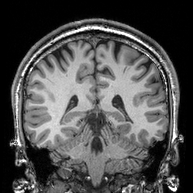
\includegraphics[width=0.99\linewidth]{texture_mri}
    \caption{\label{fig:tmri}}
  \end{subfigure}
  \begin{subfigure}{0.15\textwidth}
    
\includegraphics[width=0.99\linewidth]{texture_checkerboard}
    \caption{\label{fig:checkerboard}}
  \end{subfigure}
  \begin{subfigure}{0.15\textwidth}
    
\includegraphics[width=0.99\linewidth]{Mr}
    \caption{\label{fig:tmh}}
  \end{subfigure}
  \begin{subfigure}{0.15\textwidth}
    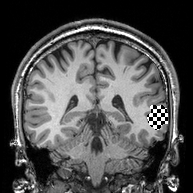
\includegraphics[width=0.99\linewidth]{texture_hard}
    \caption{\label{fig:blh}}
  \end{subfigure}
  \begin{subfigure}{0.15\textwidth}
    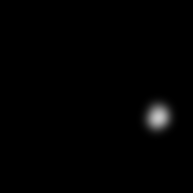
\includegraphics[width=0.99\linewidth]{texture_mask_soft}
    \caption{\label{fig:tms}}
  \end{subfigure}
  \begin{subfigure}{0.15\textwidth}
    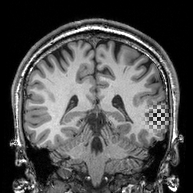
\includegraphics[width=0.99\linewidth]{texture_soft}
    \caption{\label{fig:bls}}
  \end{subfigure}

  \caption[Simulation of resected image using alpha blending]{
    Simulation of resected image $\X\simul$.
    We use a checkerboard for visualization.
    Two scalar-valued images $\X\pre$ (\subref{fig:tmri})
    and $\X_2$ (\subref{fig:checkerboard})
    are blended using $\Y\simul$ (\subref{fig:tmh})
    and $\sigma_i = \SI{0}{\milli \meter}$ to create an image with hard boundaries (\subref{fig:blh})
    and $\sigma_i = \SI{5}{\milli \meter}$ (\subref{fig:tms})
    for an image with soft boundaries (\subref{fig:bls}),
    mimicking partial-volume effects.
  }
  \label{fig:texture}
\end{figure}


\section{Results}

\subsection{Code availability}

All the code for TorchIO is available on GitHub\fnurl{https://github.com/fepegar/torchio}.
We follow the semantic versioning system \cite{preston-werner_semantic_2020} to tag and release our library.
Releases are published on the Zenodo data repository\fnurl{https://zenodo.org/} to allow users to cite the specific version of the package they used in their experiments.
The version described in this paper is \torchioversion \cite{perez-garcia_fepegartorchio_2020}.
Detailed \ac{API} documentation is hosted on Read the Docs and comprehensive Jupyter notebook tutorials are hosted on Google Colaboratory, where users can run examples online.
The library can be installed with a single line of code on Windows, macOS or Linux using the \ac{PIP} package manager: \texttt{pip install torchio}.

TorchIO has a strong community of users, with more than 1100 stars on GitHub and more than 2000 \ac{PyPI} downloads per week\fnurl{https://pypistats.org/packages/torchio} as of October 2021.


\subsubsection{Additional interfaces}

The provided \ac{CLI} tool \texttt{torchio-transform} allows users to apply a transform to an image file without using Python.
This tool can be used to visualize only the preprocessing and data augmentation pipelines and aid in experimental design for a given application.
It can also be used in shell scripts to preprocess and augment datasets in cases where large storage is available and on-the-fly loading needs to be faster.

Additionally, we provide a \ac{GUI} implemented as a Python scripted module within the \textit{TorchIO} extension available in 3D Slicer~\cite{fedorov_3d_2012}%
\fnurl{https://github.com/fepegar/SlicerTorchIO}.
It can be used to visualize the effect of the transforms parameters without any coding (\cref{fig:slicer}).
As with the \ac{CLI} tool, users can experimentally assess preprocessing and data augmentation before network training to ensure the preprocessing pipeline is suitable for a given application.

\begin{figure}
  \centering
  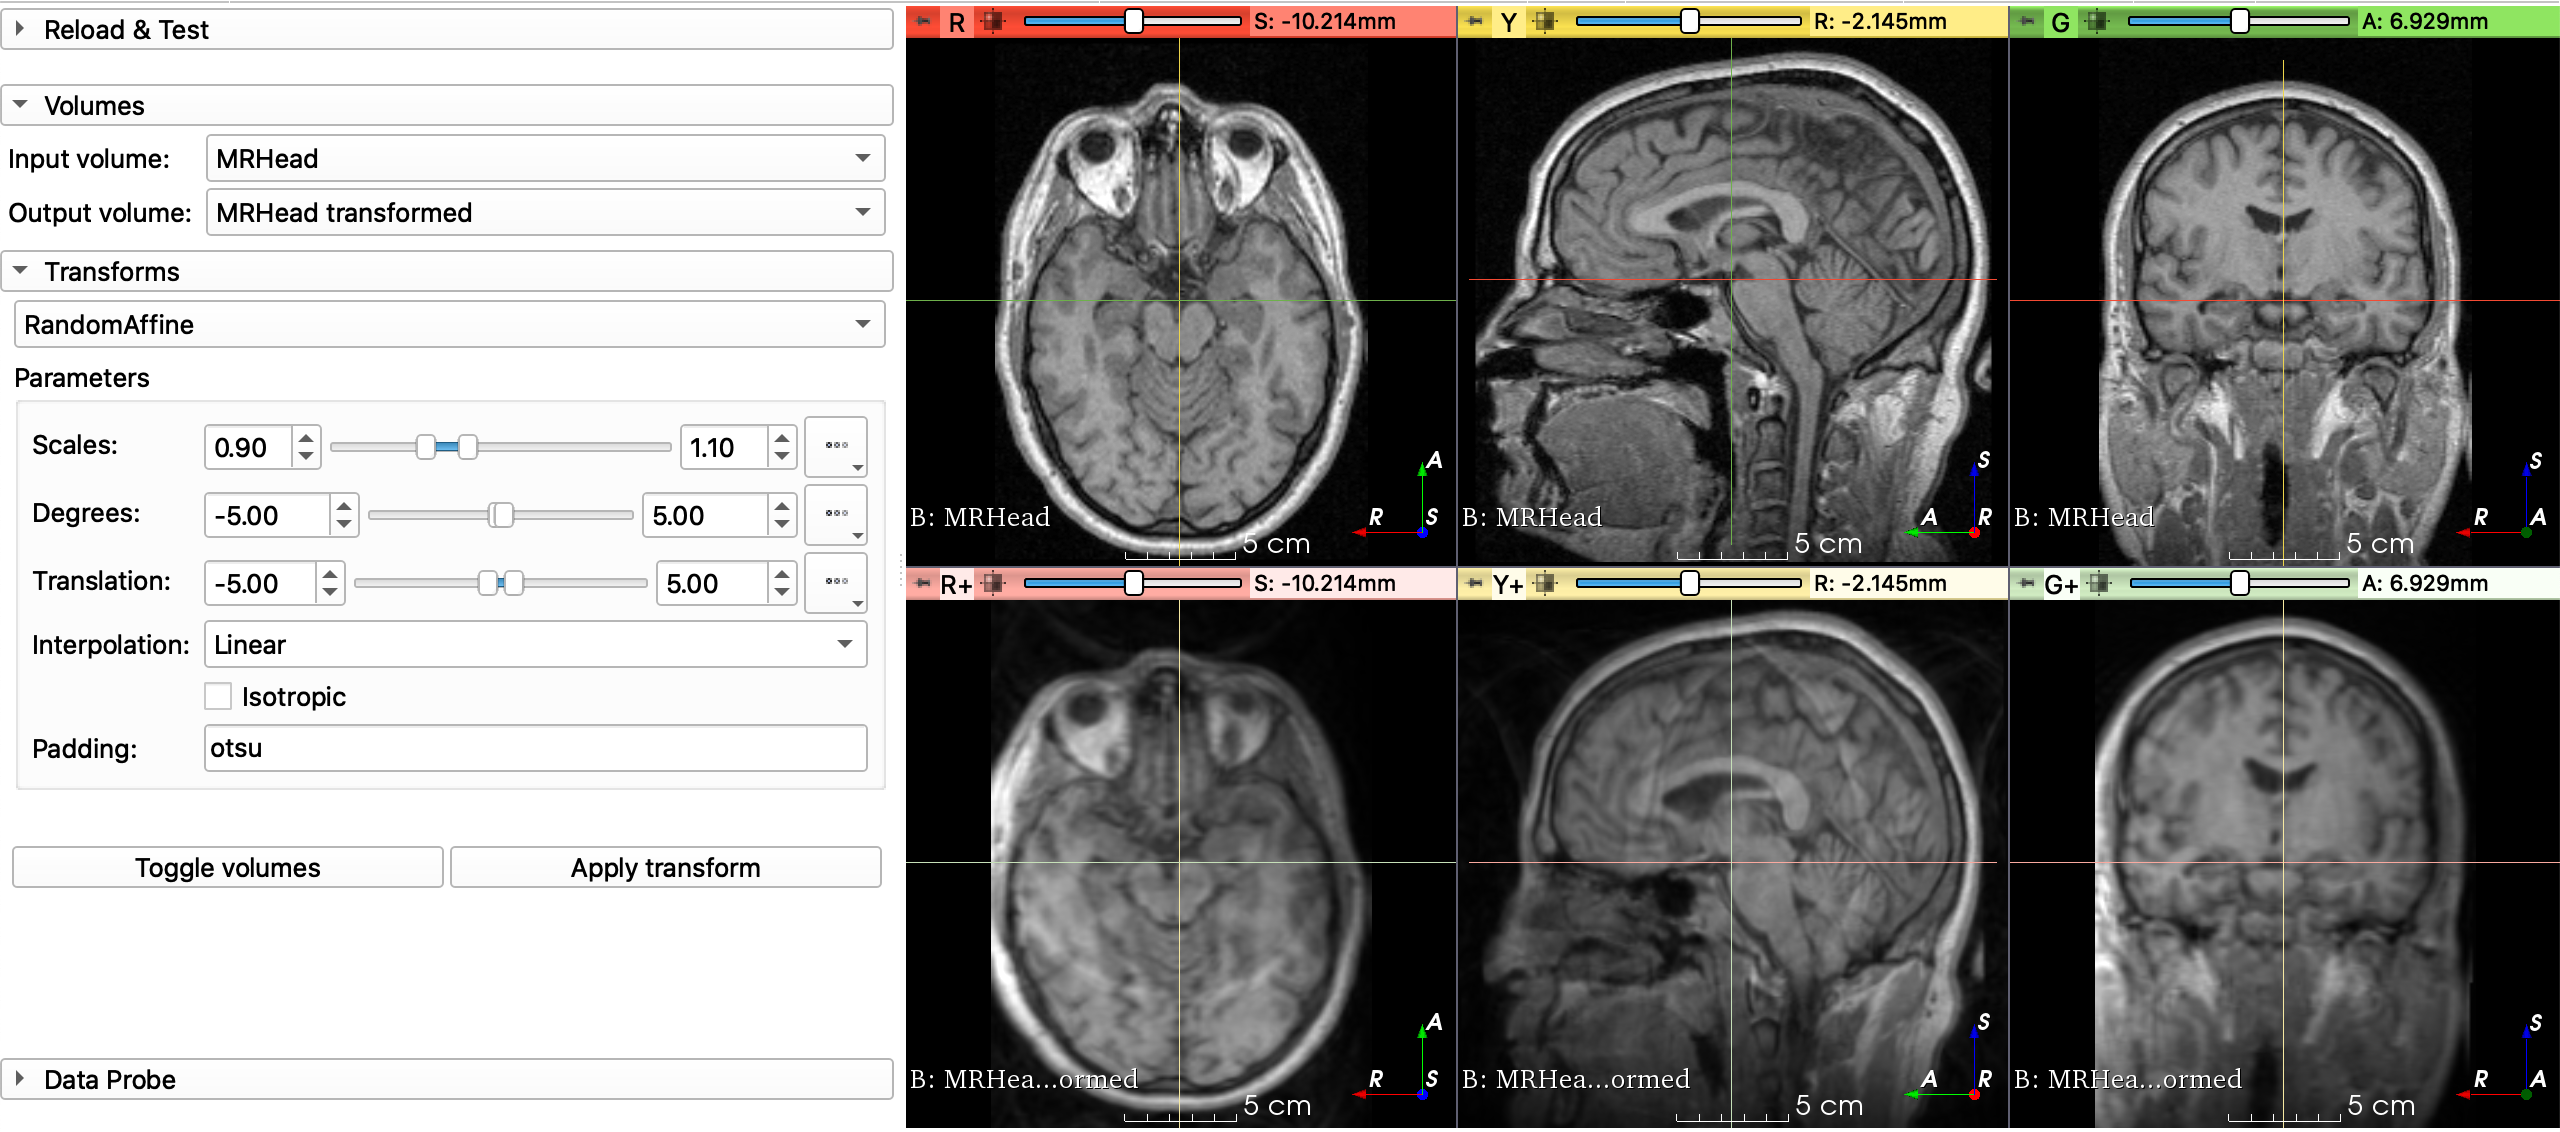
\includegraphics[width=\linewidth, trim = {0 0 0 0.1cm}, clip]{slicer}
  \caption[Graphical user interface for TorchIO]{
    \Ac{GUI} for TorchIO, implemented as a 3D Slicer extension.
    In this example, the applied transforms are
    \texttt{RandomBiasField},
    \texttt{RandomGhosting},
    \texttt{RandomMotion},
    \texttt{RandomAffine} and
    \texttt{RandomElasticDeformation}.
  }
  \label{fig:slicer}
\end{figure}

% \subsection{Usage examples}

In this section, we briefly describe the implementations of two medical image computing papers from the literature, pointing out the TorchIO features that could be used to replicate their experiments.


\subsubsection{Super-resolution and synthesis of MRI}

In \cite{iglesias_joint_2020}, a method is proposed to simulate high-resolution $T_1$-weighted \acp{MRI} from images of different modalities and resolutions.

First, brain regions are segmented on publicly available datasets of brain \ac{MRI}.
During training, an \ac{MRI} (\texttt{ScalarImage}) and the corresponding segmentation (\texttt{LabelMap}) corresponding to a specific subject (\texttt{Subject}) are sampled from the training dataset (\texttt{SubjectsDataset}).
Next, the same spatial augmentation transform is applied to both images by composing an affine transform (\texttt{RandomAffine}) and a nonlinear diffeomorphic transform (\texttt{RandomElasticDeformation}).
Then, a \ac{GMM} conditioned on the labels is sampled at each voxel location to simulate an \ac{MRI} of arbitrary contrast (\texttt{RandomLabelsToImage}) \cite{billot_learning_2020}.
Finally, multiple degrading phenomena are simulated on the synthetic image: variability in the coordinate frames (\texttt{RandomAffine}), bias field inhomogeneities (\texttt{RandomBiasField}),
partial-volume effects due to a large slice thickness during acquisition \cite{billot_partial_2020} (\texttt{RandomAnisotropy}), registration errors (\texttt{RandomAffine}), and resampling artifacts (\texttt{Resample}).


\subsubsection{Adaptive sampling for segmentation of CT scans}

In \cite{berger_adaptive_2018}, \ac{CT} scans that are too large to fit on a \ac{GPU} are segmented using patch-based training with weighted sampling of patches.
Discrepancies between labels and predictions are used to create error maps and patches are preferentially sampled from voxels with larger error.

During training, a CT scan (\texttt{ScalarImage}) and its corresponding segmentation (\texttt{LabelMap}) from a subject (\texttt{Subject}) are loaded and the same augmentation is performed to both by applying random rotations and scaling (\texttt{RandomAffine}).
Then, voxel intensities are clipped to $[-1000, 1000]$ (\texttt{RescaleIntensity}) and divided by a constant factor representing the standard deviation of the dataset (can be implemented with \texttt{Lambda}).
As the \ac{CT} scans are too large to fit in the \ac{GPU}, patch-based training is used (\texttt{Queue}).
To obtain high-resolution predictions and a large receptive field simultaneously, two patches of similar size but different \ac{FOV} are generated from each sampled patch: a context patch generated by downsampling the original patch (\texttt{Resample}) and a full-resolution patch with a smaller \ac{FOV} (\texttt{CropOrPad}).
At the end of each epoch, error maps for each subject (\texttt{Subject}) are computed as the difference between the labels and predictions.
The error maps are used in the following epoch to sample patches with large errors more often (\texttt{WeightedSampler}).
At inference time, a sliding window (\texttt{GridSampler}) is used to predict the segmentation patch by patch, and patches are aggregated to build the prediction for the whole input volume (\texttt{GridAggregator}).

% \section{Discussion}

We have presented TorchIO, a new library to efficiently load, preprocess,
augment and sample medical imaging data during the training of \acp{CNN}.
%
It is designed in the style of the deep learning framework PyTorch
to provide medical imaging specific preprocessing and data augmentation
algorithms.


The main motivation for developing TorchIO as an open-source toolkit is to help
researchers standardize medical image processing pipelines and allow them to
focus on the deep learning experiments.
%
It also encourages good open-science practices, as it supports experiment
reproducibility and is version-controlled so that the software can be cited
precisely.


The library is compatible with other higher-level deep learning frameworks for
medical imaging such as \ac{MONAI}.
%
For example, users can benefit from TorchIO's \ac{MRI} transforms and
patch-based sampling while using \ac{MONAI}'s networks, losses, training pipelines
and evaluation metrics.

\textcolor{rev2}{%
The main limitation of TorchIO is that most transforms are not differentiable.
%
The reason is that PyTorch tensors stored in TorchIO data
structures must be converted to SimpleITK images or NumPy arrays
within most transforms, making them not compatible
with PyTorch's automatic differentiation engine.
%
However, compatibility between PyTorch and ITK has recently been
improved, partly thanks to the appearance of the \ac{MONAI}
project \cite{mccormick_itk_2021}.
%
Therefore, TorchIO might provide differentiable transforms in the future, which
could be used to implement, e.g., spatial transformer networks for image
registration \cite{lee_image-and-spatial_2019}.
%
Another limitation is that many more transforms that are \ac{MRI}-specific exist than for other imaging modalities such as \ac{CT} or \ac{US}.
This is in part due to more users working on \ac{MRI} applications and requesting \ac{MRI}-specific transforms.
However, we welcome contributions for other modalities as well. 
}


In the future, we will work on extending the preprocessing and augmentation
transforms to different medical imaging modalities
such as \ac{CT} or \ac{US}, and improving compatibility with related works.
%
The source code, as well as examples and documentation,
are made publicly available online, on GitHub.
%
We welcome feedback, feature requests, and contributions to the library,
either by creating issues on the GitHub repository or by emailing the authors.
